\documentclass[border=3mm,svgnames]{standalone}
\usepackage{tkz-euclide}

\tikzset{every picture/.style = {font=\scriptsize}}

\begin{document}
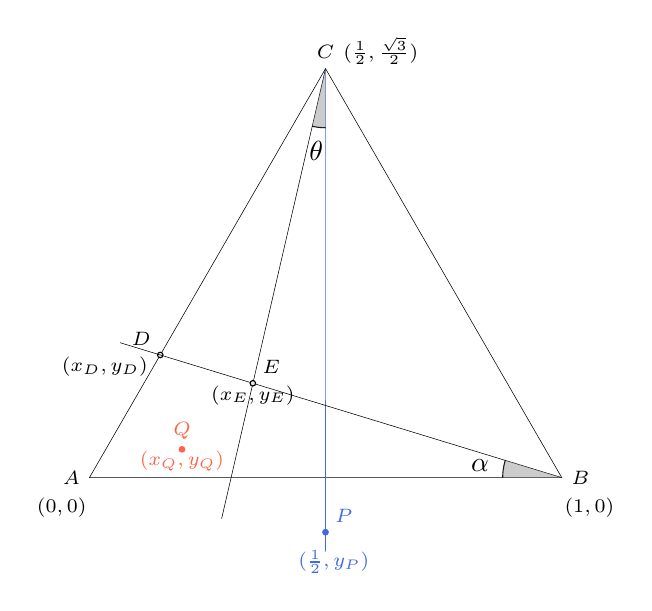
\begin{tikzpicture}[scale=1.5]
    % set up coordinates
    \tkzDefPoint(0,0){A}
    \tkzDefPoint(4,0){B}
    
    % draw equilateral ABC triangle
    \tkzDefTriangle[equilateral](A,B)\tkzGetPoint{C}
    \tkzDrawPolygon(A,B,C)
    
    % find the intersection of AB with perpendicular line from C
    \tkzDefPointBy[projection=onto A--B](C)\tkzGetPoint{H}
    \tkzDrawLines[add=0 and 0.18,RoyalBlue](C,H)
    %\tkzDrawPoints(H)
    %\tkzMarkRightAngle[size=.2, fill=gray!20, opacity=.3](B,H,C)
    % to mark angle on the outside, get point C' symmetric wrt H
    % suspend the bounding box
    %\begin{pgfinterruptboundingbox}
    %\tkzDefPointBy[symmetry=center H](C)\tkzGetPoint{C'}
    %\tkzMarkRightAngle[size=.2, fill=gray!20, opacity=.3](C',H,B)
    %\end{pgfinterruptboundingbox}

    % get a point H' on AB | case where CH is not perpendicular to AB
    \tkzDefPointOnLine[pos=0.3](A,B)\tkzGetPoint{H'}
    \tkzDrawLines[add=0 and 0.1](C,H')%\tkzDrawPoints(H')
    
    % get a point D on line AC
    \tkzDefPointOnLine[pos=0.3](A,C)\tkzGetPoint{D}
    \tkzDrawPoints(D)
    \tkzDrawLines[add=0 and 0.1](B,D)
    
    % get intersection of line BD and CH
    \tkzInterLL(B,D)(C,H')\tkzGetPoint{E}
    \tkzDrawPoints(E)
    %\tkzDrawLines[add=0 and 0.1](A,E)
    
    % first circumcircle
    \tkzDefCircle[circum](A,B,D)\tkzGetPoint{P}
    %\tkzDrawCircle[RoyalBlue](P,A)
    
    % second circumcircle
    \tkzDefCircle[circum](A,E,D)\tkzGetPoint{Q}
    %\tkzDrawCircle[Tomato](Q,A)
    
    % draw labels
    \tkzSetUpLabel[font=\scriptsize]
    \tkzLabelPoints[left](A)
    \tkzLabelPoints[right](B)
    \tkzLabelPoints[above](C)
    \tkzLabelPoints[above left](D)
    \tkzLabelPoints[above right](E)
    \tkzLabelPoints[above right,RoyalBlue](P)
    \tkzLabelPoints[above,Tomato](Q)
    \tkzText[xshift=-1em,yshift=-2.5ex](A){$(0,0)$}
    \tkzText[xshift=+1em,yshift=-2.5ex](B){$(1,0)$}
    \tkzText[xshift=+2.0em,yshift=+1.5ex](C){$(\frac{1}{2},\frac{\sqrt{3}}{2})$}
    \tkzText[xshift=-2em,yshift=-1ex](D){$(x_{D},y_{D})$}
    \tkzText[xshift=0em,yshift=-1ex](E){$(x_{E},y_{E})$}
    \tkzText[xshift=.3em,yshift=-2.5ex,RoyalBlue](P){$(\frac{1}{2},y_{P})$}
    \tkzText[xshift=0em,yshift=-1ex,Tomato](Q){$(x_{Q},y_{Q})$}

    % mark angle ABD
    \tkzMarkAngle[size=.5,fill=gray](D,B,A)
    \tkzFillAngle[fill=gray, size=.5, opacity=0.4](D,B,A)
    \tkzLabelAngle[pos=0.7](D,B,A){$\alpha$}

    % mark angle ECP
    \tkzMarkAngle[size=.5,fill=gray](E,C,P)
    \tkzFillAngle[fill=gray, size=.5, opacity=0.4](E,C,P)
    \tkzLabelAngle[pos=0.7](E,C,P){$\theta$}
    
   % draw EPQ triangle
   %\tkzDrawPolygon[LimeGreen,thin](E,P,Q)
    
    % draw circumcenters
    \tkzSetUpPoint[size=2]
    \tkzDrawPoints[RoyalBlue](P)
    \tkzDrawPoints[Tomato](Q)
    
    % shrink the bounding box
    %\tkzShowBB
    \tkzClipBB
\end{tikzpicture}
\end{document}
